\section{Entry criteria}
Due to start an integration test two constraints must be satisfied:
the major classes must be covered by ,at least , a 60 percent of unit test, 
while for the others a 30 percent is sufficient.
%TODO spiegare meglio quali siano le classi 'major'
%Ogni classe deve avere una percentuale di unit test del 60% per le classi principali,
%e il 30% per quelle derivate.

\section{Elements to be integrated}
In our case element is synonym of class; now we're going to show the classes that
need integration test in order to be sure that our application will work correctly.
\begin{itemize}
  \item[Ridesmanager]: it needs to be integrated with:
    \begin{itemize}
      \item[Ride, Sharedride]: in order to store information about the actived rides
      \item[Taxiqueue]: in order to take information of available taxis
        in case of taxi request.
      \item[Controller]: in order to exchange information about user's( and also guest's) requests
    \end{itemize}
  \item[Controller]: it needs to be integrated with:
    \begin{itemize}
      \item[User]: in order to create an ad-hoc Controller and to retrieve information about users
      \item[Servernetworkinterface]: in order to communicate with the corresponding client side
    \end{itemize}
  \item[Servernetworkinterface]: it needs to be integrated with:
    \begin{itemize}
      \item[Clientmessage]: in order to read client's messages
      \item[Servermessage]: in order to send messages to the client
    \end{itemize}
   \item[Activity]: it needs to be integrated with
     \begin{itemize}
       \item[Action]: in order to provides the allowed actions
       \item[Userinterface]: in order to provide the set of items this class needs to show
     \end{itemize}
   \item[Action]: it needs to be integrated with the Clientnetworkinterface in order to send
     requests to the server
   \item[Userinterface]: it needs to be integrated with the Clientnetworkinterface in order to
     show the right Activity according to the server message
   \item[Clientnetworkinterface]: it needs to be integrated with:
     \begin{itemize}
       \item[Clientmessage]: in order to send messages to the server 
       \item[Servermessage]: in order to read server's messages
     \end{itemize}
\end{itemize}
%Ridesmanager: Sharedride, Ride, Controller:{ User, Servornetwrokinterface },
%              Taxiqueue
%Servernetworkinterface: Clientmessage, Servermessage
%Activity: Action:{Clientnetworkinterface},Userinterface 
%Clientnetworkinterface: Clientmessage, Servermessage

\section{Integration testing strategy}
In this section we will explain how we planned the integration test
in order to build, as soon as possible, a running application 
with few working features; this will allow us to easly show
our progress to the customer, and also , in case of delay, 
to launch a working application, also with missing requirements.
In order to reach our goal we decide to apply a bottom-up method
for integration test and top down method for unit test.\\
The first working version of our application will include major classes;
in this there are no users but only a guest that has the possibility
to access all altredy implemented features.\\
The second vesrion will add the other users with realted constraints,
as explained in the previous documents ( RASD and Design Document).\\
From the second version the application could be released, considering 
that only few features are already implemented.\\
The next versions will include other features that allow us to reach
all missing requirements.
%Unit testing->Top-down
%Integration testing->bottom-up

\section{Sequence of component/Function integration}
%1- Componenti base del server: Ridesmanager, Controller, Guestcontroller
%2- Componenti base del client: Action, LoginAction, Activity, Userinterface
%   			        ^^^^^^^^^^^^^^^^^^^^^^^^^^ rivedere questa sequenza
%3- Componenti base networking: Clientnetworkinterface Servernetworkinterface,
%                               Clientmessage, Servermessage
%4- Integrazione server-client
%5- Componenti utente: User, Taxidriver, Passenger, Passengerscontroller
%                      Taxidriverscontroller, Ride
%6- Integrazione utente
%7- Fuznioni avanzate: Sharedride, Reservation
%8- Integrazione funzioni avanzate

\subsection{Software integration sequence}
\begin{figure} [h]
  \centering
  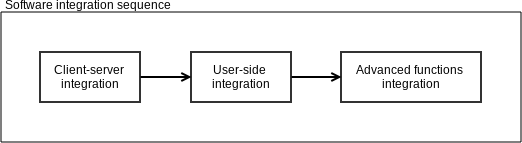
\includegraphics[scale=0.72]{diagrams/software integration.png}
  \caption{\label{fig:soft_int} Software integration}
\end{figure}
%punti: 4, 6, 8

\subsection{Subsystem integration sequence}
The classes are presented here in the ordered sequence in which they will be implemented, which is:
\ref{fig:base_serv_comp} $\rightarrow$ \ref{fig:base_client_comp} $\rightarrow$ \ref{fig:base_net_comp}
 $\rightarrow$ \ref{fig:ext_client_comp} $\rightarrow$ \ref{fig:adv_func}

Note: the arrows here represent the ordering of the implementation, which may happen to partially
match the logical structure of the class; however, those arrows do not aim to describe the inter-class
relationships

\begin{figure} [h]
  \centering
  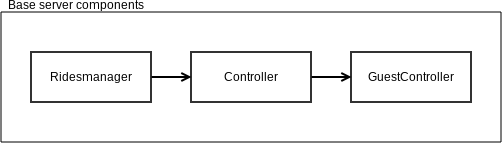
\includegraphics[scale=0.72]{diagrams/point 1.png}
  \caption{\label{fig:base_serv_comp} Base server components}
  \vspace{3mm}
  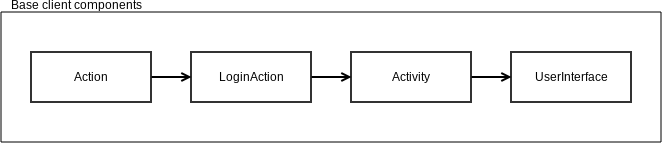
\includegraphics[scale=0.6]{diagrams/point 2.png}
  \caption{\label{fig:base_client_comp} Base client components}
  \vspace{3mm}
  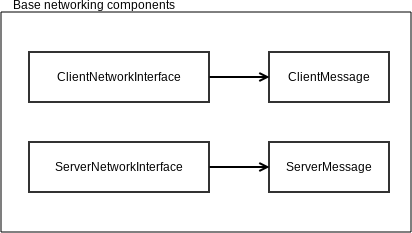
\includegraphics[scale=0.72]{diagrams/point 3.png}
  \caption{\label{fig:base_net_comp} Base networking components}
  \vspace{3mm}
  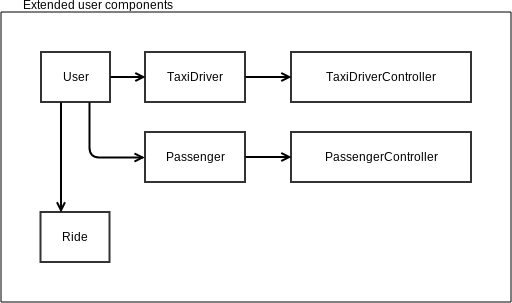
\includegraphics[scale=0.68]{diagrams/point 5.png}
  \caption{\label{fig:ext_client_comp} Extended client components}
\end{figure}
\begin{figure} [h]
  \centering
  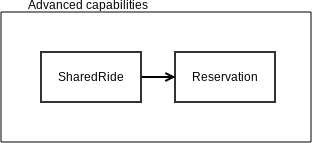
\includegraphics[scale=0.72]{diagrams/point 7.png}
  \caption{\label{fig:adv_func} Advanced functions}
\end{figure}

%punti: 1,2,3,5,7

